O presente estudo adota uma abordagem experimental e descritiva, centrada no desenvolvimento e validação inicial de um sistema de monitoramento inteligente de sono para prevenção de Acidente Vascular Cerebral (AVC) em idosos. O foco principal está no monitoramento contínuo de sinais vitais durante o sono, aliado à interpretação automatizada dos dados clínicos, de modo a fornecer subsídios para a tomada de decisão médica.

A metodologia foi estruturada em quatro etapas principais: Aquisição dos sinais fisiológicos, transmissão e armazenamento dos dados, análise e processamento inteligente e visualização e interpretação médica.\\

\begin{figure}[!htb]
\centering
\caption{Visão geral do sistema}
\label{fig:metodologia-sistema}
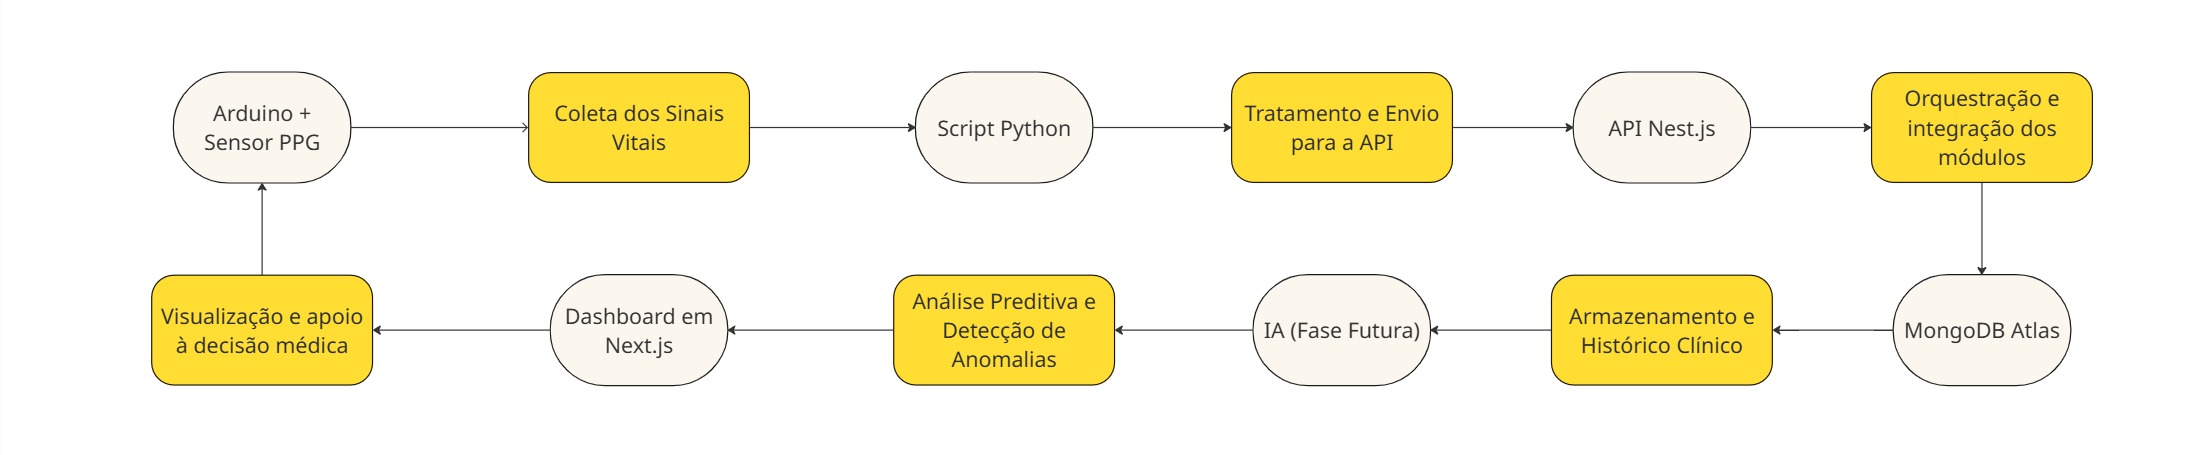
\includegraphics[width=0.8\textwidth]{Illustrations/Fluxograma.jpg}\\
\SourceOrNote{Autoria Própria (2025)}
\end{figure}

\subsection*{Aquisição dos sinais fisiológicos}

Na primeira etapa, foi utilizado um sensor de pulso cardíaco óptico acoplado a uma plataforma Arduino, responsável pela coleta contínua dos sinais de frequência e ritmo cardíaco. O sensor baseia-se no princípio da fotopletismografia (PPG), técnica óptica não invasiva que mensura variações do volume sanguíneo a partir da luz refletida pelos tecidos biológicos \parencite{TimarFulepPPG,Charlton2023}. Durante os testes laboratoriais, o dispositivo foi posicionado na extremidade do dedo do participante, possibilitando a captação precisa e ininterrupta dos batimentos por minuto (BPM) e do padrão rítmico do pulso durante o período de sono.

\subsection*{Transmissão e armazenamento dos dados}

Os dados captados pelo Arduino são transmitidos via interface serial para um computador intermediário, responsável por atuar como ponte entre o dispositivo físico e a infraestrutura de armazenamento. Nessa etapa, as informações são processadas por um script desenvolvido em Python, que executa funções de leitura contínua, filtragem de ruídos e normalização dos valores obtidos. O script também realiza a padronização temporal das amostras, garantindo a consistência das séries de dados ao longo das sessões de monitoramento.

Após a validação, os dados são estruturados em formato JSON (JavaScript Object Notation) e enviados via requisições HTTP para o servidor, onde são armazenados em um banco de dados não relacional MongoDB, hospedado em um cluster do MongoDB Atlas. Essa configuração em nuvem assegura alta disponibilidade, escalabilidade horizontal e redundância geográfica, características essenciais para sistemas de monitoramento contínuo e com potencial expansão para múltiplos usuários.

Essa estrutura de armazenamento fornece suporte robusto para futuras correlações clínicas entre variáveis fisiológicas e risco de AVC, além de servir como base de treinamento para os modelos de Inteligência Artificial planejados. A integração entre o script em Python e o banco MongoDB garante eficiência na comunicação, redução de perdas de pacotes de dados e segurança no tratamento das informações biomédicas, consolidando a arquitetura como uma fundação confiável para análises médicas baseadas em dados.

\subsection*{Orquestração e integração via API}

A comunicação entre os módulos do sistema é realizada por meio de uma API desenvolvida em Nest.js, que atua como camada de orquestração central da aplicação. Essa API é responsável por receber os dados processados em Python, armazená-los no banco MongoDB, e disponibilizá-los de forma segura e estruturada para os módulos de visualização e análise.
Além disso, a arquitetura da API segue princípios de modularidade e desacoplamento, garantindo a expansão futura para novos serviços, como a integração com modelos de IA e dashboards personalizados para diferentes perfis de usuários (médicos, cuidadores e pesquisadores). A adoção de protocolos RESTful e autenticação via tokens JWT assegura confiabilidade, segurança e rastreabilidade em todo o fluxo de dados biomédicos.

\subsection*{Análise e processamento inteligente}

Atualmente em estágio de planejamento e experimentação laboratorial, o módulo de Inteligência Artificial (IA) constitui o núcleo analítico do sistema proposto, sendo responsável por interpretar os dados biomédicos armazenados e detectar padrões anômalos relacionados à frequência e ao ritmo cardíaco. O principal objetivo dessa camada é identificar episódios de Fibrilação Atrial (FA) — um dos principais precursores de AVC isquêmico — por meio da análise de séries temporais obtidas a partir de sinais fotopletismográficos (PPG).

O desenvolvimento do módulo baseia-se na aplicação de técnicas de aprendizado supervisionado e modelos de redes neurais convolucionais (CNNs) adaptados para o tratamento de dados fisiológicos contínuos. As CNNs são particularmente adequadas para essa tarefa por sua capacidade de extrair características locais e padrões rítmicos sutis dos sinais temporais, permitindo a diferenciação entre oscilações cardíacas regulares e irregularidades compatíveis com episódios arrítmicos. Estão sendo estudadas abordagens híbridas que combinam CNNs com redes recorrentes (RNNs) ou Long Short-Term Memory (LSTM), de forma a ampliar a capacidade do modelo em capturar dependências de longo prazo presentes nas variações cardíacas noturnas.

Os resultados obtidos pela IA serão retroalimentados ao banco de dados principal, vinculados a cada paciente de forma segura e anonimizada. Essa retroalimentação permitirá a construção de um histórico clínico longitudinal, no qual cada nova análise complementa as anteriores, formando um ecossistema de aprendizado contínuo. Paralelamente, os insights gerados pelo modelo — como alertas de risco ou padrões anômalos — serão disponibilizados ao médico por meio da API central em Nest.js, que orquestra a comunicação entre os módulos de armazenamento, análise e interface visual.

No futuro, essa camada analítica permitirá a evolução do sistema de uma abordagem meramente descritiva para uma interpretação preditiva, capaz de emitir alertas automatizados em tempo quase real e oferecer apoio à decisão clínica baseada em dados. Essa integração entre IA e prática médica não apenas aprimora a precisão diagnóstica, como também potencializa a prevenção de eventos cerebrovasculares em populações de risco, consolidando o sistema como uma ferramenta de suporte clínico inteligente e escalável.

\subsection*{Visualização e interpretação médica}

A camada de visualização foi desenvolvida utilizando o framework Next.js, constituindo um dashboard clínico interativo projetado para a interpretação e acompanhamento de dados fisiológicos de pacientes idosos em monitoramento. Essa interface atua como elo direto entre os módulos tecnológicos do sistema e o profissional de saúde, transformando dados técnicos em informações clínicas de alto valor interpretativo.

O painel é composto por gráficos dinâmicos e indicadores em tempo quase real, que exibem tanto os dados brutos dos sinais vitais — como frequência cardíaca, ritmo e variação temporal — quanto as interpretações analíticas geradas automaticamente pela camada de Inteligência Artificial. Esses resultados são organizados de forma hierarquizada, permitindo ao médico alternar entre visualizações macro, que mostram tendências de longo prazo, e análises detalhadas, que possibilitam a identificação de anomalias pontuais durante o período de sono.

A arquitetura do dashboard foi estruturada com foco em usabilidade, clareza visual e precisão na comunicação dos dados clínicos, utilizando princípios de design centrado no usuário médico. Essa abordagem visa reduzir a carga cognitiva durante a análise, oferecendo recursos como filtros temporais, comparativos históricos, alertas visuais e resumos interpretativos. Dessa forma, o sistema facilita a interpretação contextualizada das informações, promovendo uma tomada de decisão mais fundamentada e eficiente.

A comunicação entre a interface e os demais módulos é orquestrada pela API central desenvolvida em Nest.js, responsável por mediar as requisições entre o banco de dados MongoDB Atlas, os scripts de processamento em Python e o módulo de IA. Essa arquitetura modular e desacoplada garante baixa latência nas consultas, consistência dos dados apresentados e alta disponibilidade do sistema, permitindo que as informações clínicas sejam acessadas com segurança e confiabilidade.

O protótipo resultante integra, de maneira coesa, todos os componentes tecnológicos do projeto — o módulo físico de captação (Arduino), o processamento de dados (Python), a API de orquestração (Nest.js), o banco em nuvem (MongoDB Atlas) e a interface médica (Next.js). Essa sinergia entre hardware, backend, infraestrutura em nuvem e inteligência artificial confere ao sistema robustez, escalabilidade e eficiência operacional, assegurando a precisão na análise dos sinais vitais e ampliando o potencial clínico do monitoramento remoto como ferramenta de apoio à prevenção de AVC em idosos.

Além disso, o dashboard não se limita a uma visualização estática, mas propõe uma plataforma dinâmica de suporte à decisão médica, em que a combinação de dados históricos, análises preditivas e alertas automáticos cria um ambiente propício à medicina personalizada e baseada em dados. Com isso, o sistema consolida-se como uma ferramenta inovadora voltada à vigilância cardíaca remota, contribuindo para a redução da mortalidade e das sequelas associadas a eventos cerebrovasculares.